\chapter{Model-Freee and Model-Based RL}

In the previous lectures we considered exclusively \textbf{Model-Free Reinforcement Learning} approaches, in which the agent learns directly from experience without building an explicit representation of the environment.
In particular, we saw how it is possible to:
learn directly a \textbf{policy} or a \textbf{value function} from experience.

In this chapter we introduce a different paradigm: \textbf{Model-Based Reinforcement Learning}.
The key idea is to explicitly learn a \textbf{model of the environment} from the observed data and to use that model for \textbf{planning}, that is, to derive a value function or a policy.

In this way, learning and planning are integrated within a single decision-making architecture.

\section{Model-Free vs Model-Based Reinforcement Learning}

In \textbf{Model-Free RL} the agent:
does not have a model of the environment,
but learns directly a value function and/or a policy from the observed transitions.

In \textbf{Model-Based RL}, instead, the agent:
\begin{compactitemize}
    \item learns an explicit model of the dynamics;
    \item uses that model to plan or simulate the future evolution;
    \item builds value functions and policies starting from the model.
\end{compactitemize}

\subsection{Advantages and Disadvantages}

Model-Based RL has several advantages:
the model can be learned through supervised learning techniques;
it is possible to quantify the uncertainty about the model;
planning can considerably reduce the number of real interactions needed.

However, it also has some disadvantages:
learning takes place in two phases (model learning and planning);
approximation errors propagate, since the final value depends both on the quality of the model and on the quality of the planning.

\section{What is a Model in Reinforcement Learning}

Formally, a model $\mathcal{M}$ is a representation of the MDP
$\langle \mathcal{S}, \mathcal{A}, \mathcal{P}, \mathcal{R} \rangle$,
parametrized by a set of parameters $\eta$.

We assume that the state space $\mathcal{S}$ and the action space $\mathcal{A}$ are known.
The model therefore approximates:
\[
\mathcal{M}_\eta = \langle \mathcal{P}_\eta, \mathcal{R}_\eta \rangle,
\qquad
\mathcal{P}_\eta \approx \mathcal{P}, \;
\mathcal{R}_\eta \approx \mathcal{R}.
\]

In particular:
\[
S_{t+1} \sim \mathcal{P}_\eta(\cdot | S_t, A_t),
\qquad
R_{t+1} = \mathcal{R}_\eta(S_t, A_t).
\]

Typically, conditional independence between transitions and rewards is assumed:
\[
\mathbb{P}(S_{t+1}, R_{t+1} | S_t, A_t)
=
\mathbb{P}(S_{t+1} | S_t, A_t)\,
\mathbb{P}(R_{t+1} | S_t, A_t).
\]

\subsection{Model Learning as Supervised Learning}

The goal of \textbf{model learning} is to estimate the parameters $\eta$ from the observed experience:
\[
\{ S_1, A_1, R_2, S_2, \dots, S_T \}.
\]

This problem can be traced back to supervised learning:
\[
(S_t, A_t) \longrightarrow (R_{t+1}, S_{t+1}).
\]

In particular:
learning $(S,A) \rightarrow R$ is a regression problem;
learning $(S,A) \rightarrow S'$ is a density estimation problem.

The procedure therefore consists of choosing a loss function (MSE, KL divergence, etc.)
and finding the parameters $\eta$ that minimize the empirical error on the experience dataset.

\subsection{Examples of Models}

There are many possible choices of model, with different levels of complexity:
\begin{compactitemize}
    \item table lookup model;
    \item linear expectation model;
    \item linear Gaussian model;
    \item Gaussian process model;
    \item deep neural network model.
\end{compactitemize}

The choice depends on the size of the state space, on the availability of data and on the trade-off between bias and variance.

\subsection{Table Lookup Model}

In the tabular case, the model consists of an explicit estimate of the transition probabilities and of the rewards.
The probabilities are obtained by counting occurrences:
\[
\mathcal{P}^\circ(s,a,s')
=
\frac{1}{N(s,a)}
\sum_{t=1}^{T}
\mathbb{1}(S_t=s, A_t=a, S_{t+1}=s').
\]

Analogously, the expected reward is estimated as an empirical mean:
\[
\mathcal{R}^\circ(s,a)
=
\frac{1}{N(s,a)}
\sum_{t=1}^{T}
\mathbb{1}(S_t=s, A_t=a)\,R_{t+1}.
\]

Alternatively, one can maintain a non-parametric memory of the observed transitions
and directly sample tuples $\langle s,a,r,s' \rangle$ from the dataset.

\subsection{Planning with a Learned Model}

Once a model $\mathcal{M}_\eta$ has been learned, we can solve the approximate MDP:
\[
\langle \mathcal{S}, \mathcal{A}, \mathcal{P}_\eta, \mathcal{R}_\eta \rangle.
\]

This can be done using any planning algorithm, including:
value iteration, policy iteration, or tree search.

The result of planning is a value function or a policy defined with respect to the learned model.

\subsection{Sample-Based Planning}

A particularly effective alternative to exact planning is \textbf{sample-based planning}.
In this approach the model is not used to compute expectations, but only to generate samples:

\[
S_{t+1} \sim \mathcal{P}_\eta(\cdot | S_t, A_t),
\qquad
R_{t+1} \sim \mathcal{R}_\eta(\cdot | S_t, A_t).
\]

The simulated transitions are then treated as real experience,
and standard model-free algorithms are applied to them, such as:
Monte Carlo control, SARSA, Q-learning.

This approach combines the flexibility of model-free RL
with the sample efficiency of model-based RL,
and it is the basis of many modern architectures that integrate learning, planning and simulation.

\section{Planning with an Inaccurate Model}

In Model-Based Reinforcement Learning planning is performed using a learned model
\[
\mathcal{M}_\eta = \langle \mathcal{P}_\eta, \mathcal{R}_\eta \rangle,
\]
which in general represents only an approximation of the real MDP
\[
\langle \mathcal{P}, \mathcal{R} \rangle.
\]

When the model is imperfect, that is
\[
\langle \mathcal{P}_\eta, \mathcal{R}_\eta \rangle \neq \langle \mathcal{P}, \mathcal{R} \rangle,
\]
the result of planning will also inevitably be limited.
In fact, planning produces a policy that is \emph{optimal for the approximate MDP}:
\[
\langle \mathcal{S}, \mathcal{A}, \mathcal{P}_\eta, \mathcal{R}_\eta \rangle,
\]
but such a policy can turn out to be suboptimal with respect to the real environment.

This leads to a fundamental principle:
\begin{quote}
\textbf{Model-based RL is only as good as the estimated model.}
\end{quote}

If the model is inaccurate, rational planning on that model still leads to wrong decisions,
since the agent is optimizing with respect to dynamics that do not correctly reflect reality.

\subsection{Consequences of Model Inaccuracy}

In the presence of modelling errors:
\begin{compactitemize}
    \item planning can amplify local errors of the model;
    \item a policy that appears optimal in the model can have poor performance in the real world;
    \item improving planning does not improve performance if the model is wrong.
\end{compactitemize}

The problem is not planning itself, but the discrepancy between model and environment.

\subsection{Possible Remedies}

There are two main strategies to deal with the use of inaccurate models.

The first consists of \textbf{resorting to model-free methods} when the model turns out to be clearly unreliable.
In this case the agent ignores the model and directly updates the value function or policy from real experience.

The second strategy is more sophisticated: \textbf{explicitly reasoning about model uncertainty}.
In a Bayesian context, instead of estimating a single model, a distribution over the possible models is maintained,
taking into account the uncertainty due to limited data.
In this way planning can balance exploitation and exploration in a more robust way.

\section{Real and Simulated Experience}

A central idea of modern Model-Based RL is the combined use of two sources of experience.

\subsection{Real Experience}

\textbf{Real experience} comes directly from the interaction with the real environment,
that is, from the true MDP:
\[
S' \sim \mathcal{P}(\cdot | S, A),
\qquad
R = \mathcal{R}(S, A).
\]

This experience is expensive (it requires real interaction) but perfectly reliable.

\subsection{Simulated Experience}

\textbf{Simulated experience} is instead generated by the learned model:
\[
S' \sim \mathcal{P}_\eta(\cdot | S, A),
\qquad
R = \mathcal{R}_\eta(S, A).
\]

These samples are cheap and potentially unlimited, but affected by modelling errors.

The idea is to exploit the strengths of both: the accuracy of real experience and the sample efficiency of simulated experience.

\section{Integrating Learning and Planning}

We can now systematically compare three paradigms.

\subsection{Model-Free Reinforcement Learning}

In Model-Free RL:
no model of the environment is built;
the agent learns directly a value function and/or a policy from real experience.

This approach is conceptually simple and robust to modelling errors,
but it often requires a large number of interactions with the environment.

\subsection{Model-Based Reinforcement Learning}

In Model-Based RL:
the agent learns a model from experience;
it uses the model to perform planning;
it derives value functions and policies starting from the model.

This approach is more sample-efficient,
but strongly dependent on the quality of the learned model.

\subsection{Dyna: Learning and Planning Together}
\begin{wrapfigure}{r}{0.3\textwidth}
    \centering
    \vspace{-10pt}
    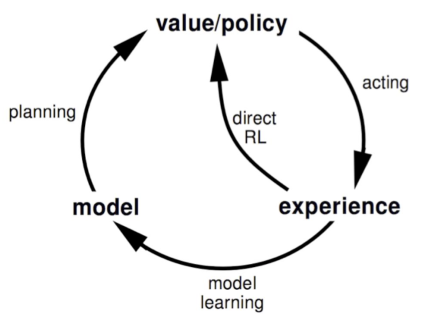
\includegraphics[width=\linewidth]{images/F1.png}
    \label{fig:Scaled Dot Product Attention}
    \vspace{-10pt}
\end{wrapfigure}
The \textbf{Dyna} architecture directly integrates learning and planning.

The agent:
\begin{compactitemize}
    \item uses real experience to update both the model and the value function (or policy);
    \item uses the model to generate simulated experience;
    \item applies model-free algorithms both to real data and to simulated data.
\end{compactitemize}

In this way:
\begin{compactitemize}
    \item real experience keeps contact with the true MDP;
    \item simulated experience speeds up learning;
    \item learning and planning take place continuously, not in separate phases.
\end{compactitemize}

Dyna therefore represents an elegant compromise between Model-Free and Model-Based RL,
and it is the basis of many modern architectures that integrate simulation, learning and real-time decision making.
\begin{figure}[H]
    \centering
    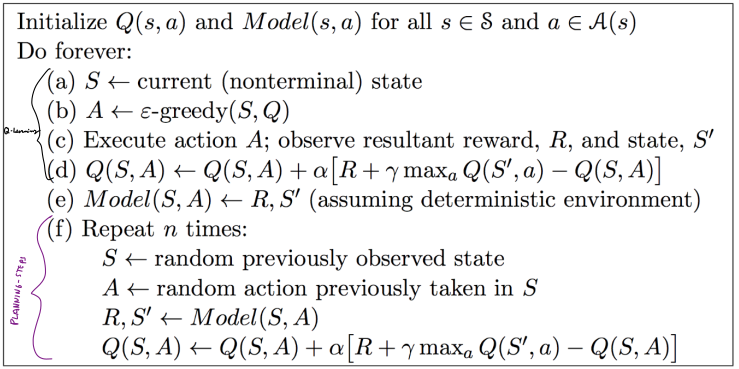
\includegraphics[width=0.8\textwidth]{images/F2.png}
    \label{fig:student_markov_chain}
\end{figure}


\section{Simulation-Based Search}

In the context of model-based RL we can use the model not to solve the whole MDP,
but only to decide which action to take \emph{now}, in the current state $s_t$.
This idea is called \textbf{simulation-based search}.

The principle is the following: instead of interacting with the real environment, we generate
fictitious episodes using the model $\mathcal{M}_\nu$ and a simulation policy $\pi$.
From these simulated episodes we estimate the values of the actions and choose the best one.

Formally, starting from $s_t$ we simulate $K$ episodes:
\[
\bigl\{\, s_t^k, A_t^k, R_{t+1}^k, \dots, S_T^k \,\bigr\}_{k=1}^K
\sim \mathcal{M}_\nu, \pi.
\]

On these $K$ episodes we can apply \emph{model-free} algorithms exactly as
if they were real experience. In practice:

\begin{compactitemize}
    \item if we apply \textbf{Monte Carlo control} to the simulated episodes we obtain
          a \emph{Monte Carlo search};
    \item if we apply \textbf{Sarsa} (or other TD methods) we obtain a form of
          \emph{TD search}.
\end{compactitemize}

So: the model is used only to generate trajectories, while the value update
remains the classic one of model-free RL.

\subsection{Simple Monte Carlo Search}

\textbf{Simple Monte Carlo Search} is the most direct version of this idea.

Suppose we have:
\begin{compactitemize}
    \item a model $\mathcal{M}_\nu$;
    \item a simulation policy $\pi$.
\end{compactitemize}

We are in the real state $s_t$ and we must choose the action $a_t$.

For \emph{each} possible action $a \in \mathcal{A}$:

\begin{enumerate}
    \item we fix the first action to $a$ and simulate $K$ episodes from the model:
    \[
    \bigl\{\, s_t^k, a, R_{t+1}^k, S_{t+1}^k, A_{t+1}^k, \dots, S_T^k \,\bigr\}_{k=1}^K
    \sim \mathcal{M}_\nu, \pi.
    \]
    The complete history of each episode is sampled jointly from the model
    (for transitions and rewards) and from the policy $\pi$ (for future actions).

    \item for each episode we compute the return starting from $t$:
    \[
    G_t^k = R_{t+1}^k + \gamma R_{t+2}^k + \dots + \gamma^{T_k - t - 1} R_{T_k}^k.
    \]

    \item we estimate the value of $a$ in $s_t$ by averaging the returns:
    \[
    Q(s_t,a)
    =
    \frac{1}{K} \sum_{k=1}^{K} G_t^k
    \;\approx\;
    q^\pi(s_t,a).
    \]
\end{enumerate}

Finally we choose the real action that maximizes this estimate:
\[
a_t = \arg\max_{a \in \mathcal{A}} Q(s_t,a).
\]

Important observations:

\begin{compactitemize}
    \item only the actions in the \emph{root state} $s_t$ are evaluated;
    \item the successor states are neither stored nor reused: each decision
          starts again from scratch at the next time-step.
\end{compactitemize}

\subsection{Monte Carlo Tree Search}

\textbf{Monte Carlo Tree Search (MCTS)} extends Simple Monte Carlo Search
by explicitly building a search tree and reusing the information
about all the visited states, not only about the root.

\subsubsection{Evaluation with MCTS}

Given a model $\mathcal{M}_\nu$ and a simulation policy $\pi$, we start from the
real state $s_t$ and once again simulate $K$ episodes:

\[
\bigl\{\, s_t^k, A_t^k, R_{t+1}^k, S_{t+1}^k, A_{t+1}^k, \dots, S_T^k \,\bigr\}_{k=1}^K
\sim \mathcal{M}_\nu, \pi.
\]

During these simulations:
\begin{compactitemize}
    \item we build a tree that contains all the visited states and actions;
    \item for each pair $(s,a)$ we count how many times it has been seen:
          $N(s,a)$;
    \item for each visit we accumulate the return $G_u^k$ starting from the time $u$
          at which the pair $(S_u^k, A_u^k)$ is equal to $(s,a)$.
\end{compactitemize}

The estimated value of $(s,a)$ is therefore:

\[
Q(s,a)
=
\frac{1}{N(s,a)}
\sum_{k=1}^{K}
\sum_{u=t}^{T_k}
\mathbf{1}\bigl( S_u^k = s,\, A_u^k = a \bigr)\, G_u^k
\;\approx\;
q^\pi(s,a).
\]

When the search ends, the real action to execute is the one that maximizes
$Q(s,a)$ in the root state:
\[
a_t = \arg\max_{a \in \mathcal{A}} Q(s_t,a).
\]

Unlike Simple Monte Carlo Search, here we reuse the simulated data to
evaluate \emph{all} the states of the subtree, not only the initial state.

\subsection{Simulation and policy improvement}

In MCTS the simulation policy $\pi$ is not fixed: it improves as
simulations accumulate. Each simulation is conceptually divided into two phases:

\begin{compactitemize}
    \item \textbf{in-tree phase}: as long as we are in nodes already present in the tree,
          the action is chosen with a \emph{tree policy} (for example $\epsilon$-greedy
          on $Q(s,a)$), which balances exploration and exploitation;
    \item \textbf{out-of-tree phase}: when we reach a new state, the tree is
          expanded and from there on a simpler \emph{default policy} is followed,
          typically random.
\end{compactitemize}

After each simulated episode, the values $Q(s,a)$ are updated with Monte Carlo
evaluation and the tree policy is gradually made more greedy with respect to these values.
In practice we are applying \textbf{Monte Carlo control} to the experience
generated by the model; under suitable conditions the estimates converge to:
\[
Q(S,A) \longrightarrow q^*(S,A)
\]
on the explored tree.

In summary:
\begin{compactitemize}
    \item Simple Monte Carlo Search evaluates only the actions in the current state;
    \item Monte Carlo Tree Search builds and updates an entire search tree,
          reusing the same simulated experience for many states and actions.
\end{compactitemize}
\begin{figure}[H]
    \centering
    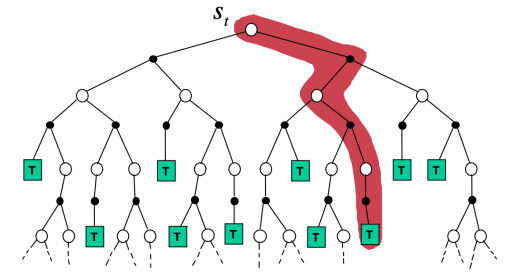
\includegraphics[width=0.8\textwidth]{images/F3.png}
    \label{fig:student_markov_chain}
\end{figure}